\documentclass[12pt, a4paper]{article}
\title{\textbf{Assignment 1, CS698U: Multi layer perceptron}}
\author{Nishit Asnani, 14433}
\date{January, 2017}
\usepackage[]{geometry}
\usepackage[]{graphicx}
\usepackage[]{url}
\usepackage[T1]{fontenc}
\geometry{a4paper, left=15mm, top=20mm, right=15mm, bottom=20mm,}


\begin{document}
\maketitle

\section{Objective}
To implement and understand the backpropagation algorithm by building a hand written digit classifier for the MNIST dataset with standard split.

\section{Setup}
The code has been broken up into three files:

\begin{itemize}
\item \textit{input.py}: This file is used for loading the MNIST dataset from Yann Lecun's website and storing it in a manner usable by our MLP. For this purpose, input code from \textbf{TensorFlow} tutorial's \textit{convolutional.py} (\url{https://github.com/tensorflow/tensorflow}) has been used as it is, so that obtaining the dataset in a convenient format becomes easy. 

\item \textit{mlp.py}: This file defines the class \texttt{Multi\_layer\_perceptron}, which forms the crux of the assignment. An object of this class is an MLP model, with a given number of hidden layers, number of neurons in each hidden layer, and activation function as arguments to the constructor. The various class members have been described later on in the report.

\item \textit{calling.py}: This forms a python script that loads the dataset by calling the relevant functions in \textit{input.py}, builds models using \textit{mlp.py} and trains them, recording the accuracy and loss statistics after each epoch. 

\end{itemize}

\section{Class \texttt{Multi\_layer\_perceptron}}
\begin{itemize}
\item The constructor takes number of hidden layers, number of nodes (neurons) in each hidden layer (as a list), and the activation function to be used (0 for $tanh$ and 1 for $ReLU$ as input. It initializes the relevant class members, and also initializes dictionaries corresponding to the parameters (weights), node activations, gradients, square gradients (for ADAM), and records of the previous gradient update (for GD with momentum). It also initializes geometrically decreasing estimates for $\beta_1$ and $\beta_2$, as required by ADAM. 

\item \texttt{forward\_pass} computes a forward pass through the network on a given input image and stores the node activations at each node.

\item \texttt{nonlinear} is a routine to compute non-linearity on a list of inputs according to the activation function specified.

\item \texttt{softmax} is a routine that computes the softmax probabilities of each of the output states, given the node activations in the final layer for an input image. 

\item \texttt{compute\_loss} computes the softmax loss for a given input and adds that to the class member \textit{loss}.

\item \texttt{compute\_gradients} takes the true label of the processed image, and computes the back propagated error at each node, as well as the gradient of the loss with respect to each parameter in the network. The sum of all gradients over a mini batch is constrained to be at most 5 times the batch size, to cure the problem of exploding gradients. 

\item \texttt{apply\_gd\_optimizer} uses simple gradient descent to update the weights.

\item \texttt{apply\_momentum\_optimizer} applies gradient descent with a standard momentum term to update the parameters. It uses the dictionary storing previous weight updates for this purpose. 

\item \texttt{apply\_adam\_optimizer} applies the ADAM optimizer with standard settings of $\beta_1$ and $\beta_2$ by default, but these can be passed as an argument by the \textit{train} function. It uses the accumulated average gradient and accumulated squared average gradient for this purpose. 

\item \texttt{train} takes train and validation data, and a choice of optimizer (sgd, momentum or adam) and performs training for one epoch on the training data, followed by a test on the validation dataset. It returns the loss and accuracy on the validation dataset. Except for standard GD, all the optimizers work for a stochastic minibatch setting, since it converges faster. 

\item \texttt{numerical\_gradients} takes a set of data points and computes backpropagated error of the weights on those points. Then, one parameter is perturbed slightly, and its effect on the new loss is seen after a forward pass. This is used to compute the numerical gradient of the loss with respect to that parameter, and this is done for all the parameters one after another.
 
 
\end{itemize}

\section{Experiments and Findings}
\begin{itemize}
\item I used \texttt{numerical\_gradients} to compute numerical gradients of a 2 hidden layer, (100, 25) model with ReLU activation, and plotted the mean difference and the mean squared difference between the calculated numerical gradients and the backpropagated gradients of weights lying between each successive pair of layers. The mean difference was small, and to confirm the fact that the actual difference is also small, the mean squared error also turned out to be small. 

\begin{figure}[h!]
\centering
\includegraphics[width=12cm, height=6cm]{num_back_grads_relu.eps}
\caption{Plot of mean difference between the two gradients for the parameters against the pair of layers they were connecting}
\end{figure}

Also, I looked at the individual differences as well, and they clearly lay in two main zones for a perturbation of 0.0001, indicating the firing of some neurons in ReLU while the others stayed at zero.


\begin{figure}[h!]
\centering
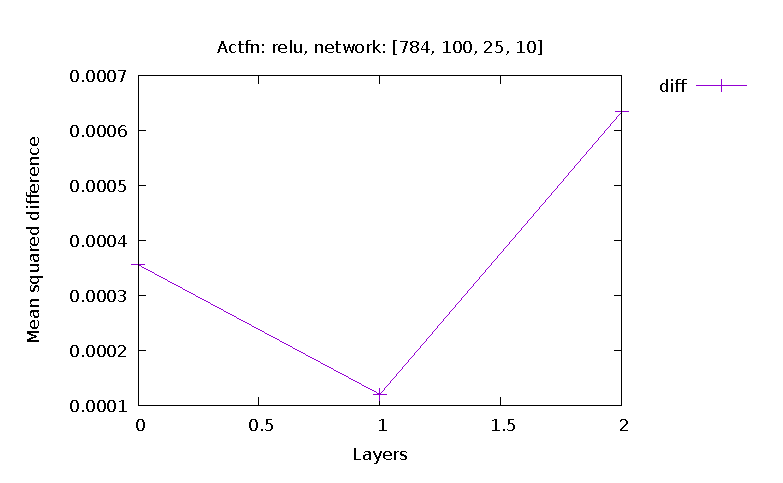
\includegraphics[width=12cm, height=6cm]{num_back_grads_relu_var.eps}
\caption{Plot of mean squared difference between the two gradients for the parameters against the pair of layers they were connecting}
\end{figure}

\item To find out the optimum activation function, I made 1 hidden layer models for both tanh and ReLU, comprising of 100, 25 and 5 nodes in the hidden layer. This also gave me an idea of a good number of neurons (while being not too time consuming to train) to keep in the first layer in a multi hidden layer neural network. 

\textbf{Note: The accuracy reported in the following figures is validation set accuracy. The minibatch size is 64, and the number of training epochs are 10.}

\begin{figure}[h!]
\centering
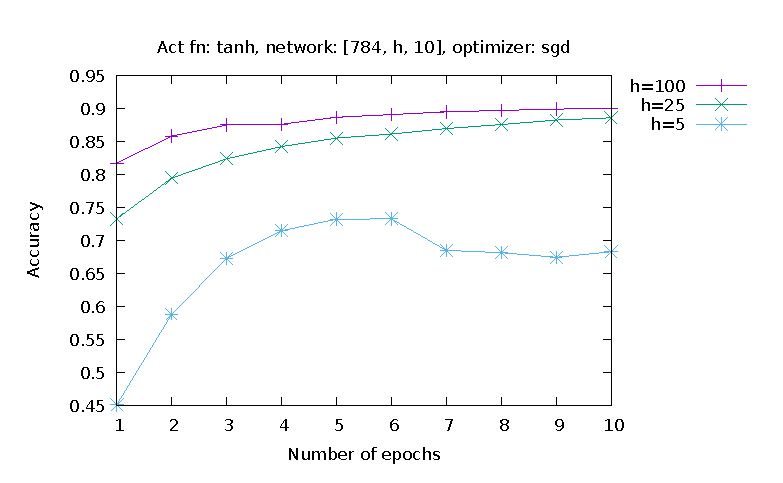
\includegraphics[width=12cm, height=6cm]{tanh_single_hidden_layer.eps}
\caption{Performance of various single hidden layer neural network architectures with the tanh activation function. }
\end{figure}

\begin{figure}[h!]
\centering
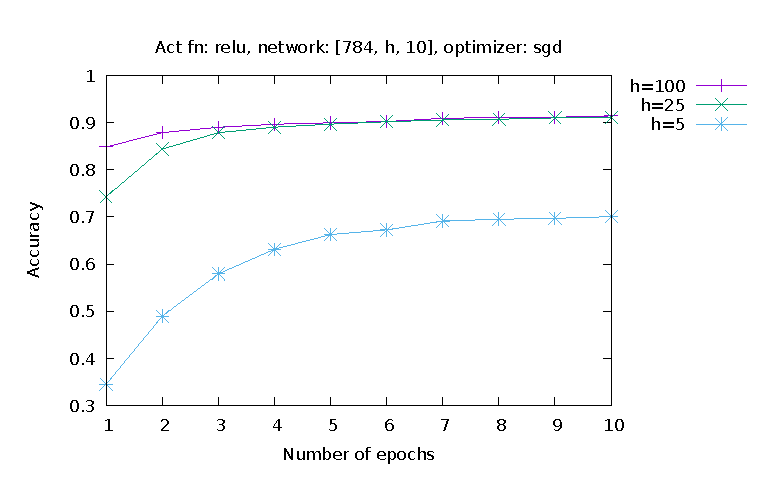
\includegraphics[width=12cm, height=6cm]{relu_single_hidden_layer.eps}
\caption{Performance of various single hidden layer neural network architectures with the relu activation function. }
\end{figure}

\begin{figure}[h!]
\centering
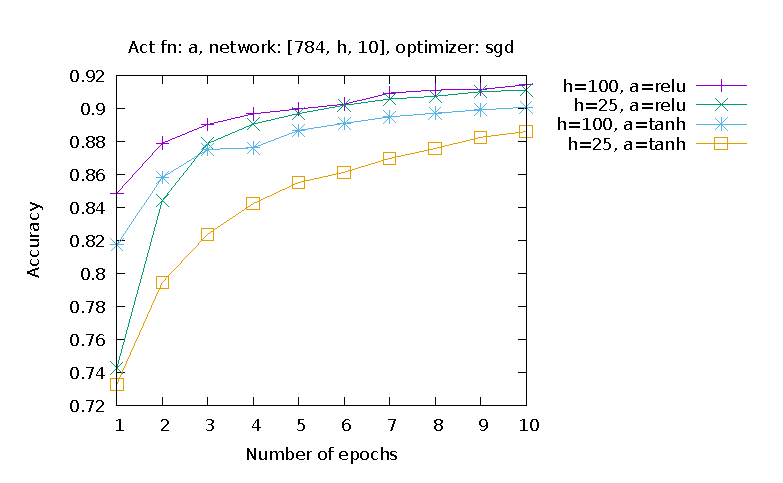
\includegraphics[width=12cm, height=6cm]{relu_tanh_single_hidden_layer.eps}
\caption{Comparative Performance of various single hidden layer neural network architectures with the relu and tanh activation functions. }
\end{figure}

Clearly, optimization happened far quicker when ReLU was used, so I decided to stick with it in further experiments.

\item The next test was to choose the best optimizer in a minibatch setting (since it became clear after a couple of tests that stochastic minibatch optimization converged far quicker than a full batch optimizer). The candidates I considered were (and those that I implemented) SGD, SGD with momentum and ADAM. With ReLU activation function, the following results were obtained:

\begin{figure}[h!]
\centering
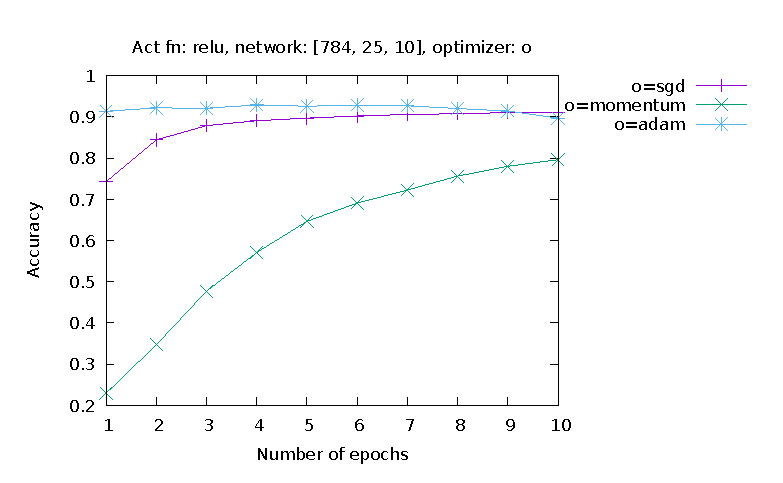
\includegraphics[width=12cm, height=6cm]{relu_25_opts.eps}
\caption{Performance of various optimizers in the given setting (25 neurons in middle layer). }
\end{figure}

\begin{figure}[h!]
\centering
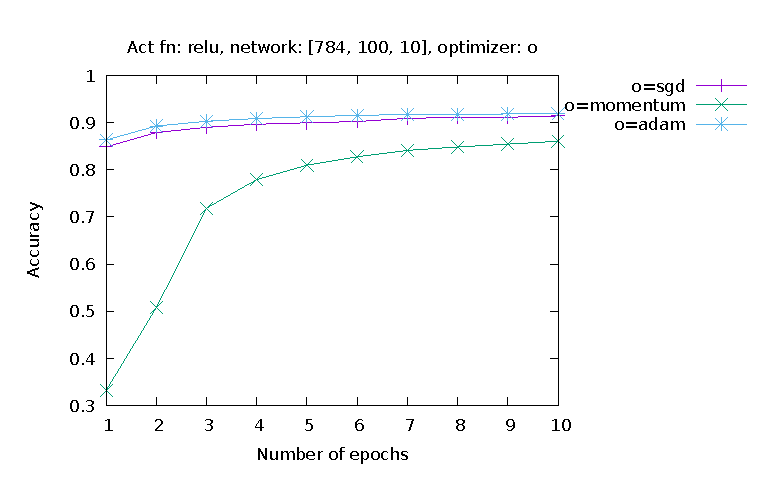
\includegraphics[width=12cm, height=6cm]{relu_100_opts.eps}
\caption{Performance of various optimizers in the given setting (100 neurons in middle layer). }
\end{figure}

\begin{figure}[h!]
\centering
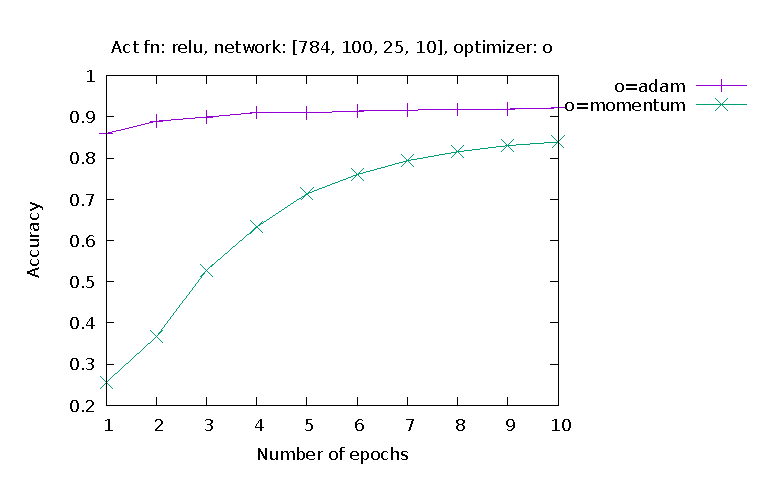
\includegraphics[width=12cm, height=6cm]{relu_100_25_opts.eps}
\caption{Performance of various optimizers in the given setting (100, 25 neurons in the second and third layer respectively). }
\end{figure}

The learning rates for the various optimization algorithms were fixed after some experimentation, ensuring that they don't diverge within the number of epochs in which the tests were conducted (10) and that they hopefully converge. Clearly, ADAM outperformed the other optimizers both in terms of accuracy at the end of 10 epochs of training as well as speed of learning in terms of number of epochs. It was slower in running time though.

\item Finally, I tested deeper networks with ReLU as the activation function and  ADAM as the optimizer for optimum performance. I started right from no hidden layer to 4 hidden layers, and plotted validation accuracy against number of hidden layers.

\begin{figure}[h!]
\centering
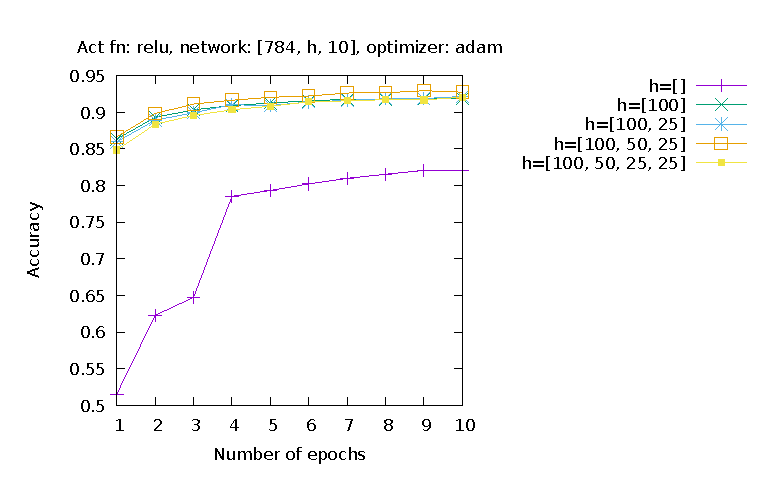
\includegraphics[width=15cm, height=8cm]{relu_multi_hidden_layer.eps}
\caption{Performance of the network as a function of network depth }
\end{figure}

In my tests, the five layer network (with three hidden layers) performs the best, but the tests are subject to a lot of other hyperparameters not tested, like the learning rate, batch size and the number of epochs.

\textbf{Note}: Figures depicting loss as a function of number of epochs (instead of accuracy) for the validation set have been included in the submission, but are not a part of this report. They can be looked at for reference.

\end{itemize}

\bibliography{ref}
\bibliographystyle{plain}
\end{document}